% EF5342 Week 5 — The Stock Market
% Beamer conversion from week5_StockMarket.pptx (59 source slides -> 38 frames).
% Compile: pdflatex week5_StockMarket.tex
% Each frame carries a [src: ...] comment mapping back to source slides
% (the content-coverage checklist; S = section divider slide in the pptx).
\documentclass[aspectratio=169]{beamer}
\usepackage{../ef5342}

\title{EF5342 Financial Systems, Markets and Instruments}
\subtitle{Week 5 --- The Stock Market}
\author{Prof.\ Weikai Li}
\institute{City University of Hong Kong}
\date{Semester B 2026--2027}

\begin{document}

% ============ STOCKS AND SHAREHOLDER RIGHTS ============

% [src: 1]
% Title-slide background art (slide01_img.jpg / slide01_img0.jpg) dropped — decorative.
\begin{frame}
\titlepage
\end{frame}

% [src: 2]
\begin{frame}{Outline}
Topics covered:
\begin{itemize}
  \item Key features of stocks
  \item Primary stock market
  \item Secondary stock market
  \item Stock return calculation
  \item Stock market indexes
  \item Stock market regulation
\end{itemize}
\end{frame}

% [src: 3]
\begin{frame}{What Are Stocks?}
Stocks represent a piece of \textbf{ownership} in a corporation; shareholders are the legal owners.
\begin{description}
  \item[Profit sharing] Right to share in the firm's profits (e.g., through dividends --- although not guaranteed)
  \item[Residual claimants] Paid only after all other claims are satisfied in the event of bankruptcy or liquidation
  \item[Limited liability] Lose only the amount invested in the stock
  \item[Control] Control the firm's activities indirectly by exercising voting rights (e.g., to elect the board of directors)
\end{description}
\end{frame}

% [src: 4]
\begin{frame}{Common vs.\ Preferred Stock}
\begin{description}
  \item[Common stock] The fundamental ownership claim in a public or private corporation. Dividends are discretionary and thus not guaranteed; holders have the lowest priority in bankruptcy and liquidation (the residual claim)
  \item[Preferred stock] Priority over common stock in payment of dividends and in liquidation. Generally fixed dividends paid quarterly; generally no voting rights unless dividend payments are missed
\end{description}
\vspace{0.3em}
Two features of preferred:
\begin{itemize}
  \item \textbf{Nonparticipating}: dividend is fixed regardless of any increase or decrease in the issuing firm's profits
  \item \textbf{Cumulative}: missed dividend payments go into arrears and must be made up before any common stock dividends can be paid
\end{itemize}
\end{frame}

% [src: 5, 6]
\begin{frame}{Shareholder Meetings, Votes, and Proxy Voting}
Publicly traded companies hold annual (or special) shareholder meetings (AGMs) to vote on important issues: election of board directors, approval of executive compensation (say-on-pay), mergers and major transactions, ratification of auditors, and shareholder proposals (e.g., on ESG issues).
\vspace{0.3em}

\textbf{Proxy voting} --- a written authorization for someone else to vote your shares --- is the standard method: most shareholders cannot or do not attend in person (meetings can be virtual, hybrid, or in-person), and \textbf{over 95\%} of votes in large public companies are cast by proxy.
\vspace{0.3em}

\begin{table}
\centering
\footnotesize
\begin{tabular}{p{0.20\textwidth}p{0.72\textwidth}}
\toprule
\textbf{Aspect} & \textbf{Impact} \\
\midrule
Corporate governance & Shareholders influence board composition, strategy, and accountability \\
Institutional power & Large funds (BlackRock, Vanguard, State Street) control huge votes via proxy \\
Activism & Enables shareholder proposals on climate, diversity, executive pay, etc. \\
Outcomes & Can sway close votes on contentious issues (e.g., director elections, mergers) \\
\bottomrule
\end{tabular}
\end{table}
\end{frame}

% [src: 7]
\begin{frame}{Proxy Contest and Shareholder Activism}
A \textbf{proxy contest} (proxy fight / proxy battle) is a shareholder-driven campaign to gain influence or control over a company by soliciting votes (proxies) from other shareholders --- usually in opposition to the existing management or board.
\vspace{0.3em}
\begin{itemize}
  \item \textbf{Triggered by dissatisfaction}: activists believe the company is underperforming, has poor governance, misallocated capital, or needs strategic change (sell the company, spin off divisions, replace CEO, cut costs)
  \item \textbf{Main goal}: replace some or all board members with the activists' own nominees (a ``board contest'') or push through specific proposals
  \item \emph{Video example:} \textbf{Other People's Money} --- management pitch vs.\ activist pitch
\end{itemize}
\end{frame}

% [src: 8]
\begin{frame}{Why Initiate a Proxy Contest?}
Shareholders are more likely to initiate a proxy contest after a period of \textbf{poor stock performance}. The chart plots cumulative abnormal returns from 24 months before the announcement of a proxy contest to 24 months after.
\begin{figure}
\centering
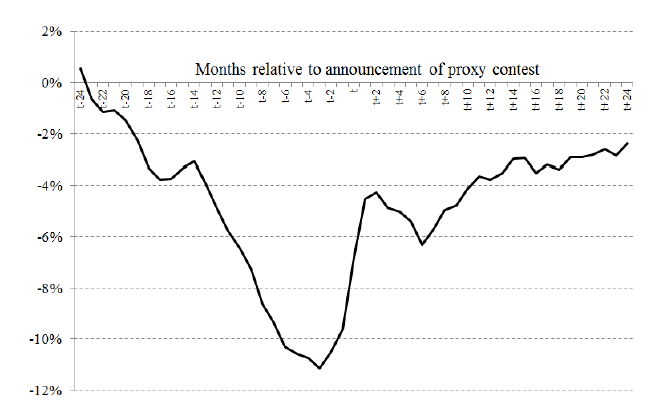
\includegraphics[height=0.54\textheight,keepaspectratio]{figures/slide08_img0.png}
\end{figure}
\begin{center}
\small Source: Fos (2016)
\end{center}
\note{https://sites.google.com/a/bc.edu/vyveslav-fos/home/proxy-contests (Vyacheslav Fos's proxy contests page).}
\end{frame}

% [src: 9, 10]
\begin{frame}{Mini Case: David Webb --- HK Pioneer of Activist Investing}
\begin{columns}
\begin{column}{0.26\textwidth}
\begin{figure}
\centering
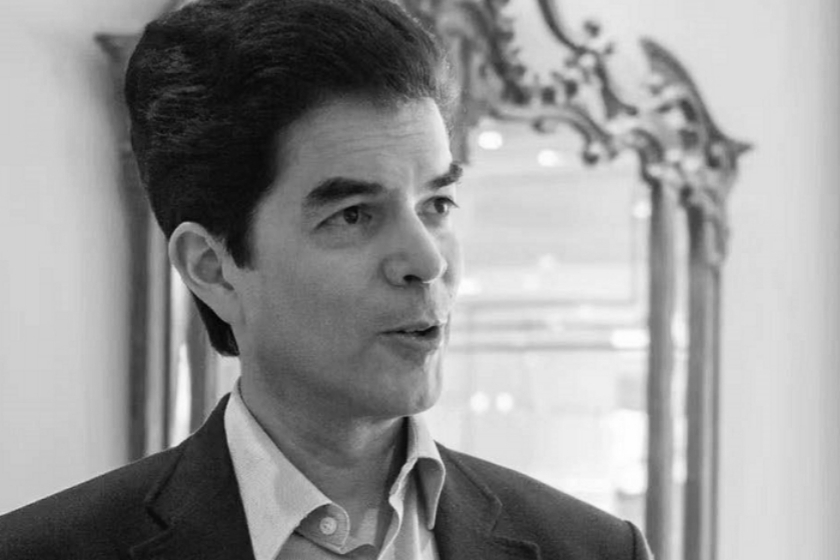
\includegraphics[height=0.28\textheight,keepaspectratio]{figures/slide09_img0.jpg}
\end{figure}
\end{column}
\begin{column}{0.70\textwidth}
\small
British-born activist investor and transparency advocate, a legendary figure in Hong Kong finance. His campaigns targeted practices that disadvantaged minority shareholders --- share dilution and opaque networks.
\begin{itemize}
  \item \textbf{Project VAMPIRE (2003)}: opposed resolutions letting companies issue up to 20\% new shares for cash without pre-emptive rights, letting controlling shareholders dilute minority stakes. Webb mobilized investors via webb-site.com; the limit was later cut to 5\% without a shareholder vote
  \item \textbf{The Enigma Network expose (2017)}: revealed 50 interconnected HK-listed companies --- brokers, construction firms, even an umbrella manufacturer --- linked by cross-shareholdings and common owners that propped up stock prices. 38 stocks plunged, some by over 90\%, wiping out billions
\end{itemize}
\end{column}
\end{columns}
\end{frame}

% ============ PRIMARY STOCK MARKETS ============

% [src: 11]
\section{Primary Stock Markets}

% [src: 12, 13]
\begin{frame}{Primary Markets and Equity Issuance}
Primary markets are markets in which corporations raise funds through \textbf{new issues of stock}, most of the time through investment banks, which act either as:
\begin{description}
  \item[Best efforts underwriting] The underwriter acts as an agent to sell the shares on behalf of the company, using their ``best efforts'' to market and sell them
  \item[Firm commitment underwriting] The underwriter buys the entire issue from the company at a discounted price and resells it to the public, assuming full ownership and risk
\end{description}
Sometimes a \textbf{syndicate} (a group of investment banks) is formed to issue stock --- the lead underwriter is the \emph{originating house}, and risk is spread among all participants.
\vspace{0.3em}

\textbf{Types of issuance:}
\begin{itemize}
  \item \textbf{IPO}: the first public issue of financial instruments by a firm --- raises money to fund operations and provides liquidity for existing shareholders to sell
  \item \textbf{SEO}: the sale of additional securities by a firm whose securities are already publicly traded
  \item \textbf{Shelf registration}: multiple issues over a two-year period with only one registration statement, so the company can time the sales to favorable market conditions
\end{itemize}
\end{frame}

% [src: 14, 15]
\begin{frame}{Benefits of IPO --- and US Equity Issuance}
\begin{columns}
\begin{column}{0.44\textwidth}
IPO benefits the firm by:
\begin{itemize}
  \item Raising additional funds for expansion, now and in the future through SEOs
  \item Public stock usable as compensation to attract talent
  \item Price discovery through secondary market trading
  \item Prestige of being a public firm may reduce the cost of borrowing
\end{itemize}
\end{column}
\begin{column}{0.54\textwidth}
\begin{figure}
\centering
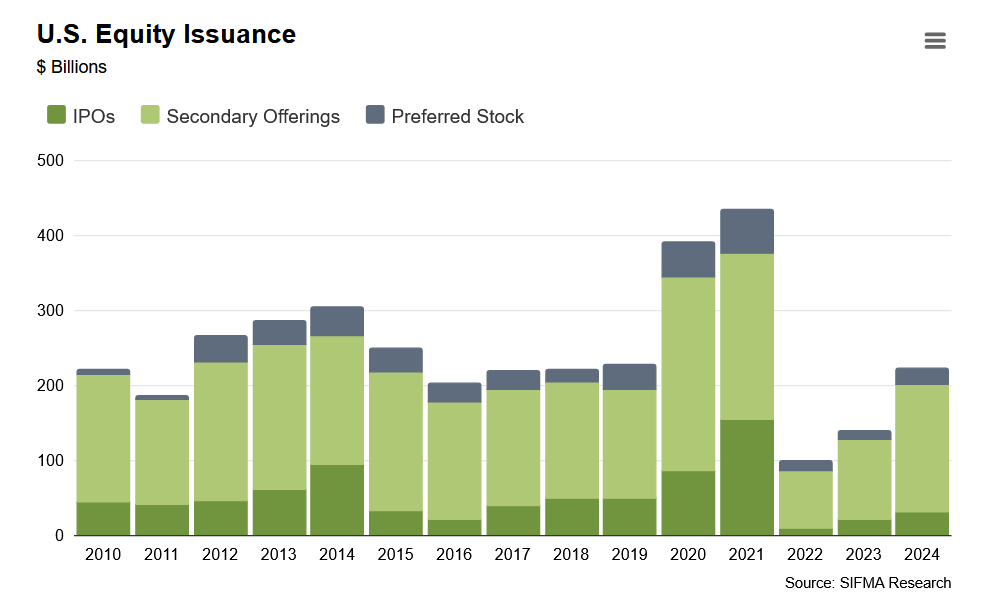
\includegraphics[height=0.55\textheight,keepaspectratio]{figures/slide15_img0_flat.png}
\end{figure}
\end{column}
\end{columns}
\end{frame}

% [src: 16]
\begin{frame}{The IPO Process}
\begin{enumerate}
  \item \textbf{Decision and preparation}: the firm decides to issue and sends a registration statement to the SEC
  \item \textbf{Preliminary prospectus distribution}: the Red Herring prospectus is sent to prospective buyers
  \item \textbf{SEC review and feedback}: the SEC requests changes or additional information
  \item \textbf{SEC evaluation / waiting period}
  \item \textbf{Final approval and offering}: the official prospectus is issued
\end{enumerate}
\begin{figure}
\centering
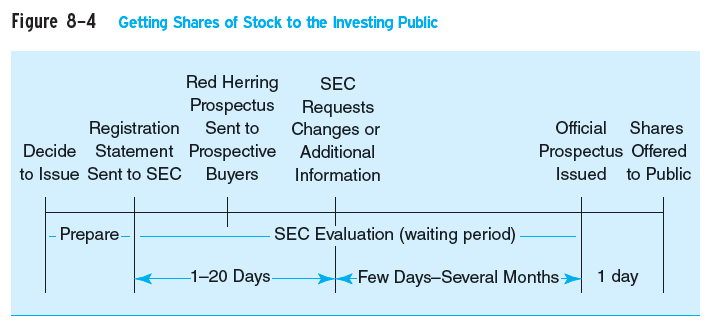
\includegraphics[height=0.42\textheight,keepaspectratio]{figures/slide16_img0.png}
\end{figure}
\note{A red herring prospectus is a preliminary version of the prospectus that describes a new security issue.}
\end{frame}

% [src: 17]
\begin{frame}{Example: An IPO Prospectus}
\begin{figure}
\centering
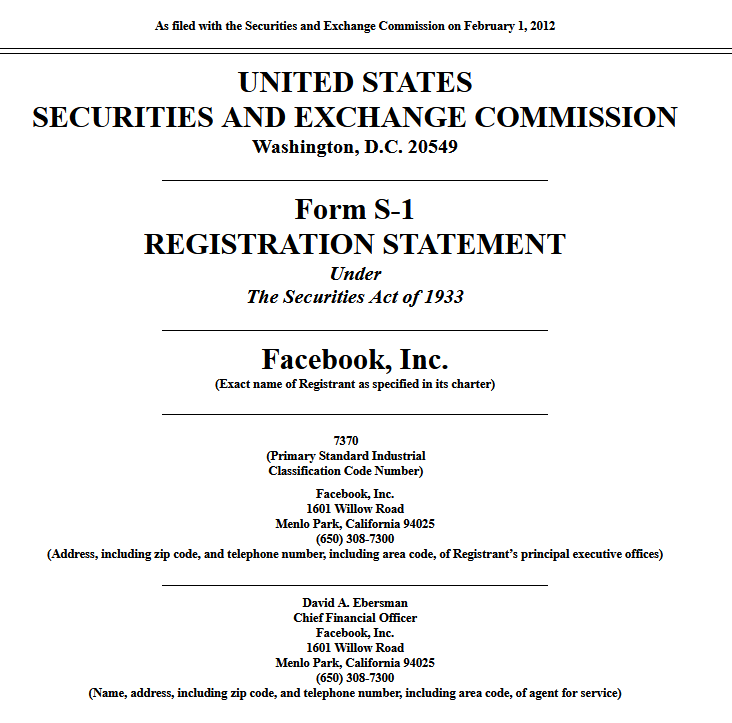
\includegraphics[height=0.72\textheight,keepaspectratio]{figures/slide17_img0_flat.png}
\end{figure}
\begin{center}
\small Source: SEC EDGAR
\end{center}
\note{https://www.sec.gov/Archives/edgar/data/1326801/000119312512034517/d287954ds1.htm}
\end{frame}

% [src: 18]
\begin{frame}{Well-Known Facts about IPOs}
\begin{description}
  \item[Underpricing of IPOs] First-day returns of IPOs are typically highly positive. The IPO firm effectively ``left money on the table'': it could have priced the offering higher and raised more money
  \item[Hot and cold markets] The number of IPOs follows hot and cold markets --- firms try to time the market, selling equity to the public when valuations are high
  \item[Long-run underperformance] IPOs perform poorly compared with similar firms 3--5 years after the IPO
\end{description}
\end{frame}

% [src: 19, 20, 21, 22]
\begin{frame}{First-Day Returns of IPOs: US, Japan, China, Hong Kong}
\begin{center}
\begin{columns}
\begin{column}{0.48\textwidth}
\centering
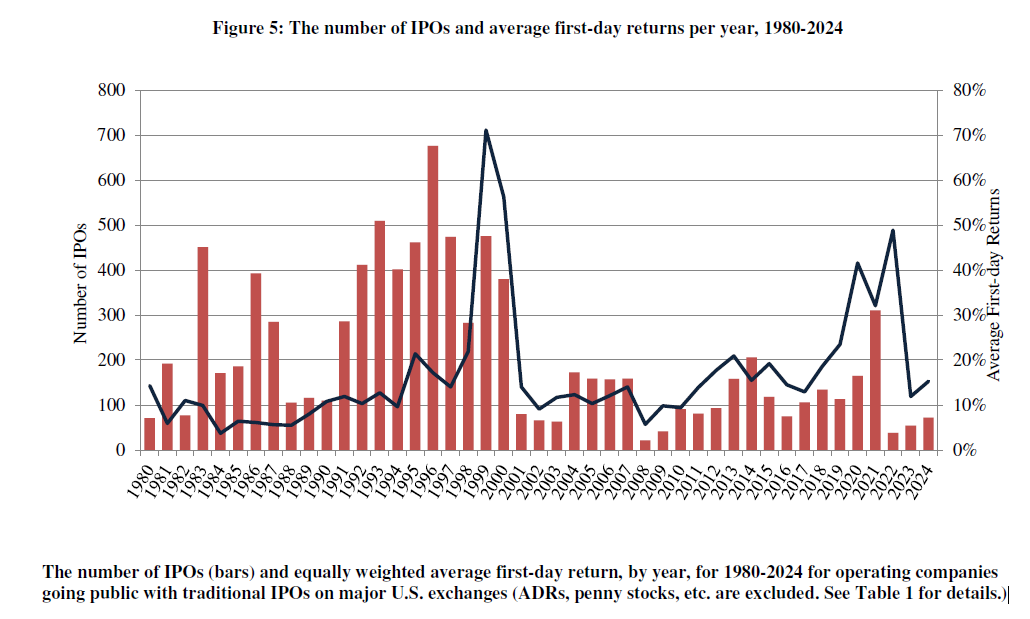
\includegraphics[height=0.33\textheight,keepaspectratio]{figures/slide19_img0_flat.png}\\
{\scriptsize US}
\end{column}
\begin{column}{0.48\textwidth}
\centering
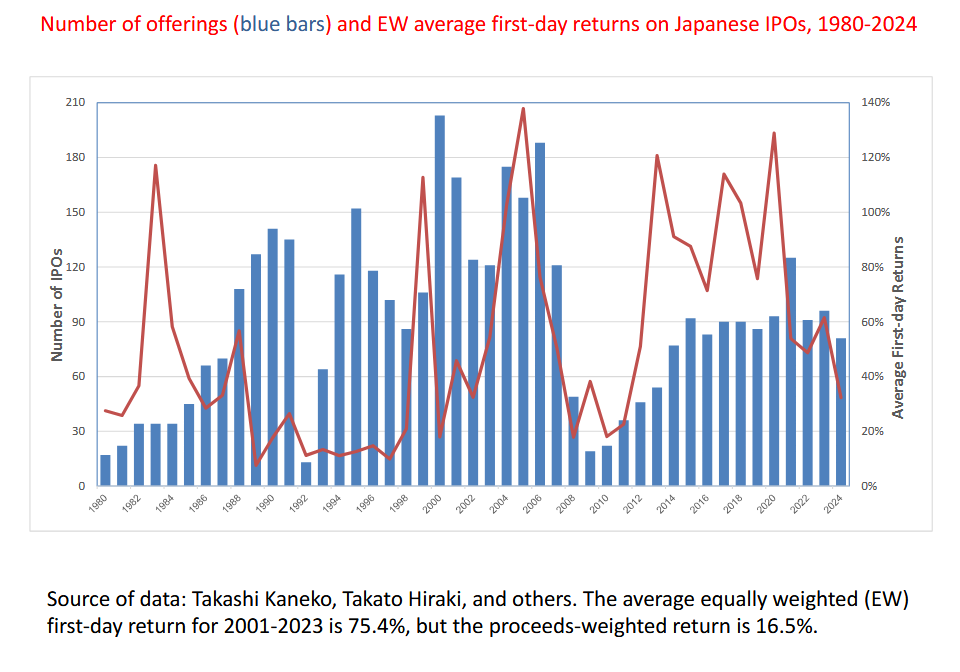
\includegraphics[height=0.33\textheight,keepaspectratio]{figures/slide20_img0_flat.png}\\
{\scriptsize Japan}
\end{column}
\end{columns}
\begin{columns}
\begin{column}{0.48\textwidth}
\centering
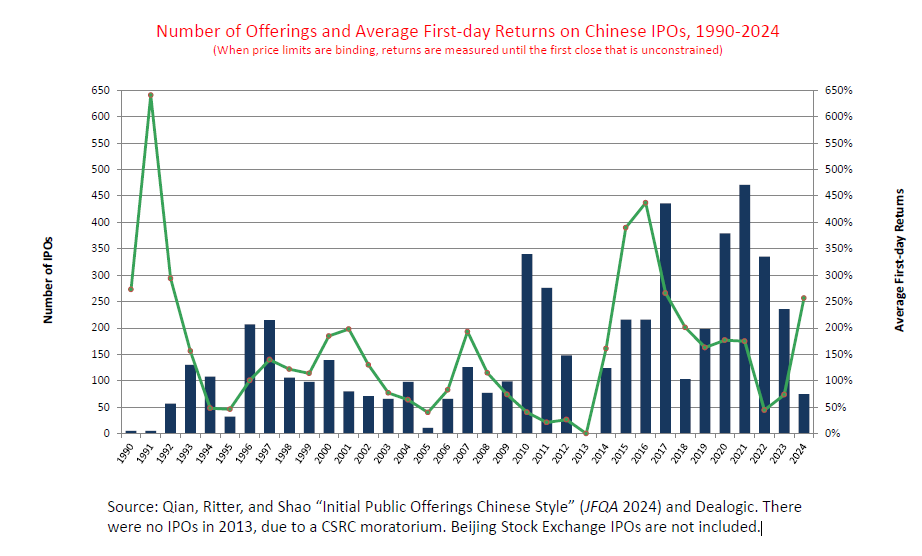
\includegraphics[height=0.33\textheight,keepaspectratio]{figures/slide21_img0_flat.png}\\
{\scriptsize China}
\end{column}
\begin{column}{0.48\textwidth}
\centering
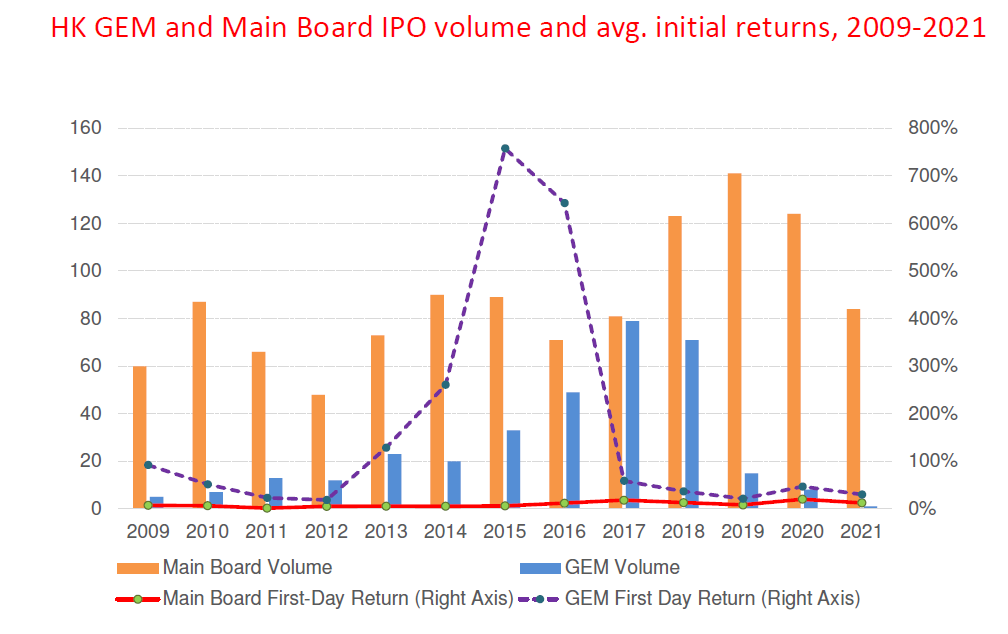
\includegraphics[height=0.33\textheight,keepaspectratio]{figures/slide22_img0_flat.png}\\
{\scriptsize Hong Kong}
\end{column}
\end{columns}
\small Source: Prof.\ Jay Ritter's website
\end{center}
\end{frame}

% [src: 23]
\begin{frame}{Why Are IPOs Underpriced? (1/2)}
\begin{description}
  \item[1. Winner's curse] Informed investors apply only if the IPO is underpriced. Uninformed investors know they will get IPO shares only when informed investors don't want to invest --- so the uninformed never want to participate. Since the firm needs to raise capital from both informed and uninformed investors, IPOs must on average be underpriced to get the uninformed to apply
  \item[2. Bandwagon hypothesis] The firm underprices to get the first few investors to participate; subsequent investors blindly follow the first few --- a story about information cascades. This generates more demand for the IPO, and more underpricing
\end{description}
\end{frame}

% [src: 24]
\begin{frame}{Why Are IPOs Underpriced? (2/2)}
\begin{description}
  \item[3. Investment bank conflicts of interest] Banks have superior information and the power to underprice IPOs. They allocate IPOs to their favorite clients and expect future favors from them. Evidence: for hot issues, underwriters set up personal brokerage accounts for venture capitalists and executives of issuing firms in order to allocate hot IPOs to them
  \item[4. Lawsuit / litigation avoidance] People who made money are less likely to examine the prospectus for false statements, and less likely to sue the firm or the investment bank when the stock underperforms later
  \item[5. Irrational investors] Overoptimistic investors pay too much for the IPO on the first day of trading --- consistent with evidence of poor long-run future performance
\end{description}
\note{Lawsuit/litigation avoidance: the underwriter deliberately underprices the IPO to ensure that even if there is a misstatement or omission, purchasers do not have a claim, since these failures are priced in the IPO.}
\end{frame}

% [src: 25, 26]
\begin{frame}{Long-Run Performance of IPOs}
IPO firms on average \textbf{underperform peer firms 3--5 years after the IPO}.
\begin{center}
\begin{columns}
\begin{column}{0.48\textwidth}
\centering
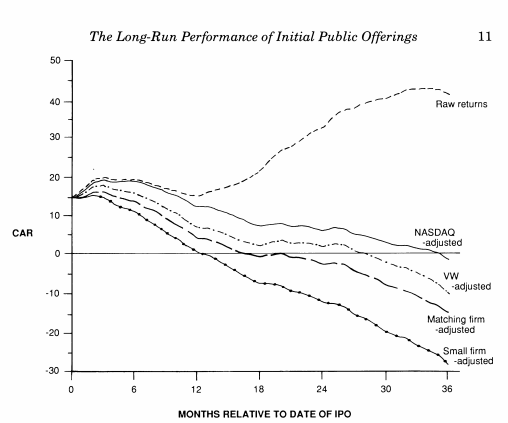
\includegraphics[height=0.42\textheight,keepaspectratio]{figures/slide25_img0.png}
\end{column}
\begin{column}{0.48\textwidth}
\centering
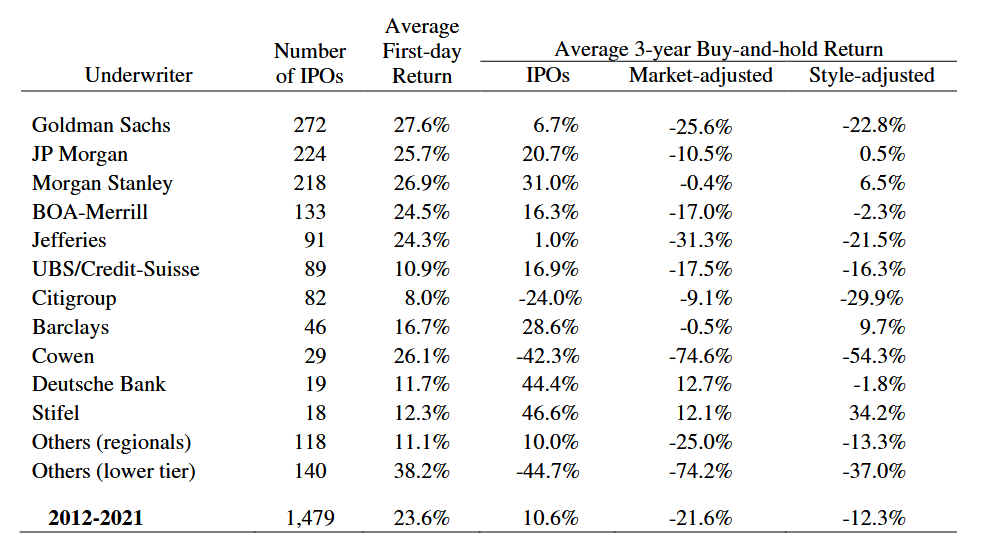
\includegraphics[height=0.42\textheight,keepaspectratio]{figures/slide26_img0_flat.png}
\end{column}
\end{columns}
\small Source: Jay Ritter (1991, \emph{Journal of Finance})
\end{center}
\end{frame}

% [src: 27]
\begin{frame}{Why Long-Run Underperformance?}
\begin{description}
  \item[Convergence of opinion] Only optimistic investors buy on the first day; pessimistic investors cannot short. Subsequently the pessimists' views get incorporated and the price drops
  \item[Passing of a fad] Investors slowly realize the firm's potential was overstated --- e.g., the technology bubble (peaking in 2000)
  \item[Firms timing the IPO market] Firms do an IPO during times when their equity is the most overvalued
  \item[IPO as lottery] Investors pay a high price hoping the stock becomes the next superstar with a huge payoff (think Google, IPO 2004; Facebook, IPO 2012)
\end{description}
\end{frame}

% [src: 28, 29]
\begin{frame}{The Decline of US Public Markets}
\begin{columns}
\begin{column}{0.42\textwidth}
\begin{figure}
\centering
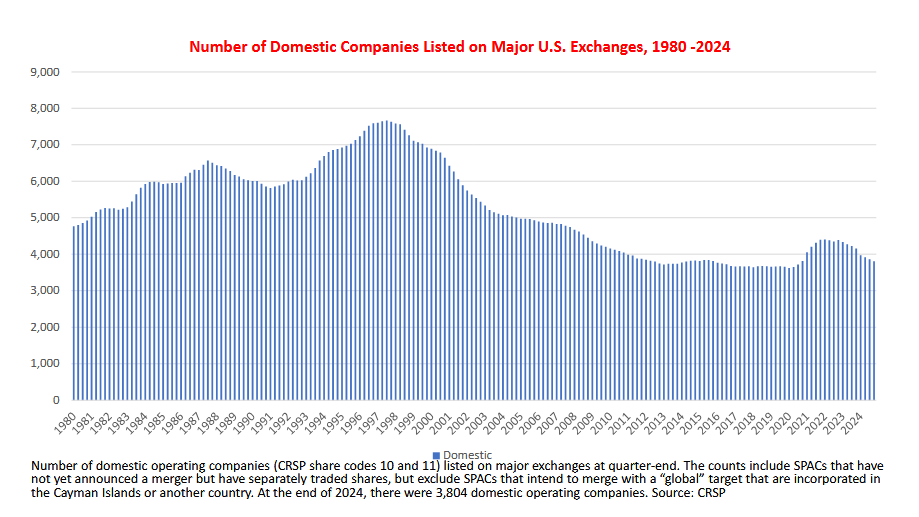
\includegraphics[height=0.42\textheight,keepaspectratio]{figures/slide28_img0_flat.png}
\end{figure}
\begin{center}
\small Source: Jay Ritter's website
\end{center}
\end{column}
\begin{column}{0.54\textwidth}
What caused the decline?
\begin{itemize}
  \item \textbf{Increasing regulatory and compliance costs}: the Sarbanes-Oxley Act of 2002, enacted in response to corporate scandals like Enron (2001), imposed stricter financial reporting, auditing, and governance requirements
  \item \textbf{Availability of private capital}: easier access to venture capital and private equity allows firms to grow without an IPO
  \item \textbf{M\&A activity}: a surge in M\&A has consolidated the market, with larger public companies acquiring smaller ones, reducing the number of independent listed firms
  \item \textbf{Decline in new listings}: fewer companies pursue IPOs due to the high upfront costs
\end{itemize}
\end{column}
\end{columns}
\end{frame}

% ============ SECONDARY STOCK MARKETS ============

% [src: 30]
\section{Secondary Stock Markets}

% [src: 31]
\begin{frame}{Secondary Stock Markets}
Secondary stock markets are the markets in which stocks, once issued, are \textbf{traded among investors}.
\begin{description}
  \item[New York Stock Exchange] Largest stock exchange in the world by market capitalization (\$32.3 trillion in listed equity at end-2025, WFE). Located on Wall Street in New York; founded in 1817; approximately 2,100 listed companies (WFE, end-2025)
  \item[NASDAQ] The world's first electronic market; no physical trading floor; heavily weighted toward technology companies
  \item[Over-the-counter (OTC) markets] A decentralized dealer network where trades occur directly between parties through broker-dealers, rather than on a centralized exchange
\end{description}
\note{ICE: Intercontinental Exchange. Bats was acquired by CBOE in 2017.}
\end{frame}

% [src: 32]
\begin{frame}{Trading on the NYSE vs.\ NASDAQ}
The NYSE and NASDAQ differ significantly in trading mechanisms, structure, and order execution.
\begin{itemize}
  \item \textbf{NYSE}: trading occurs at a specific place on the exchange floor called a \textbf{trading post}. Each stock has a special market maker --- a \emph{specialist} (old) or \textbf{Designated Market Maker} (new) --- that maintains liquidity for the stock at all times; DMMs stabilize order flows and prices in turbulent market environments
  \item \textbf{NASDAQ}: primarily a \textbf{dealer market} where multiple dealers act as market makers for a particular stock. Investors are not buying from and selling to one another directly, but through a dealer
\end{itemize}
\note{DMM: https://www.nyse.com/market-model; https://www.nyse.com/publicdocs/nyse/listing/fact\_sheet\_dmm.pdf (underscores escaped for LaTeX)}
\end{frame}

% [src: 33]
\begin{frame}{NYSE vs.\ NASDAQ}
\begin{table}
\centering
\footnotesize
\begin{tabular}{p{0.17\textwidth}p{0.36\textwidth}p{0.36\textwidth}}
\toprule
\textbf{Aspect} & \textbf{NYSE} & \textbf{NASDAQ} \\
\midrule
Primary model & Auction + Designated Market Maker (DMM) & Dealer / multiple competing market makers \\
Trading venue & Hybrid (electronic + floor presence) & 100\% electronic, no physical floor \\
Liquidity provision & DMM has affirmative obligation to provide liquidity and stabilize & Market makers compete; no single obligated party \\
Spreads \& volatility & Often tighter spreads, lower volatility (especially large-caps) & Can have wider spreads in less liquid stocks; historically higher volatility \\
Typical company & Larger, established ``blue-chip'' firms (IBM, Coca-Cola, JPMorgan) & Tech, growth, biotech, newer companies (Apple, Tesla, Amazon, NVIDIA) \\
Listed companies & $\sim$2,100 (WFE, end-2025) & $\sim$3,300 (WFE, end-2025) \\
Perception & More traditional / prestigious & More innovative / tech-oriented \\
\bottomrule
\end{tabular}
\end{table}
\end{frame}

% [src: 34, 35]
\begin{frame}{Order Types: Market vs.\ Limit Orders}
{\small
\textbf{Market order} --- buy 100 shares of AAPL right now: executes instantly at the current ask (e.g., \$225.40, even if you saw \$225.10 seconds ago).
\textbf{Limit order} --- buy AAPL only at \$220 or lower: executes only if sellers bring the price down to \$220 (or better, like \$219.50); if it never hits \$220, no trade.}
\vspace{0.2em}
\begin{table}
\centering
\scriptsize
\begin{tabular}{p{0.14\textwidth}p{0.38\textwidth}p{0.38\textwidth}}
\toprule
\textbf{Aspect} & \textbf{Market Order} & \textbf{Limit Order} \\
\midrule
Definition & Buy or sell immediately at the best available current market price & Buy or sell only at a specific price (or better) that you set \\
Execution & Almost immediately during market hours & Only if the market reaches your price (or better); may not execute at all \\
Price guarantee & None --- you get whatever the market offers (could be worse than expected in volatile conditions) & Yes --- won't pay more (buys) or receive less (sells) than your limit price \\
Execution guarantee & High --- almost always fills quickly unless extremely illiquid & None --- if the price never hits the limit, the order won't fill (may partially fill) \\
Speed & Very fast --- prioritizes immediacy & Immediate if price already met; otherwise may take days or never fill \\
Best for & Liquid stocks/ETFs; entering or exiting right away; stable markets; unconcerned about slippage & Controlling the exact price; volatile markets; target entry/exit; avoiding paying too much or selling too low \\
\bottomrule
\end{tabular}
\end{table}
\end{frame}

% [src: 36]
\begin{frame}{Circuit Breakers}
\textbf{Circuit breakers} are imposed trading halts that give investors time to make informed decisions during volatile market conditions.
\vspace{0.3em}

During March 2020, the S\&P 500 plunged sharply, triggering circuit breakers \textbf{four times in just 10 trading days} --- an extremely rare event.
\begin{figure}
\centering
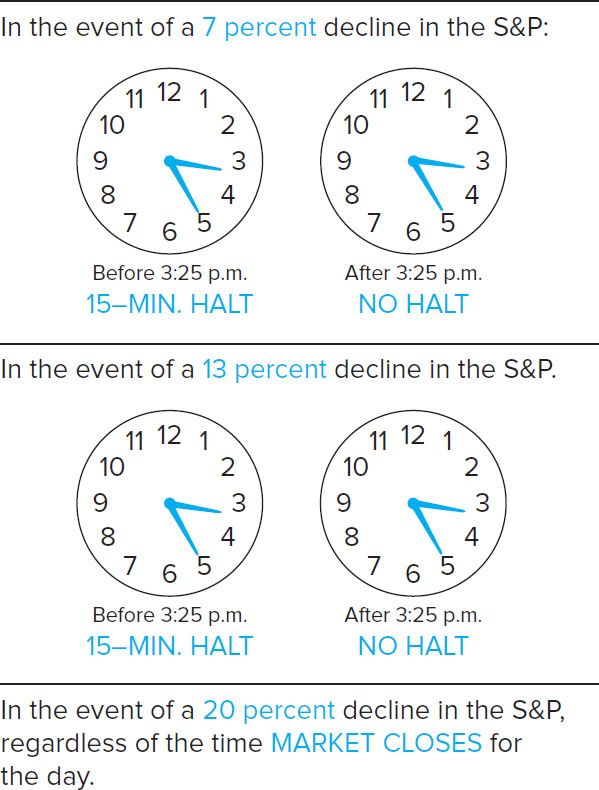
\includegraphics[height=0.50\textheight,keepaspectratio]{figures/slide36_img0.jpg}
\end{figure}
\begin{center}
\small Source: New York Stock Exchange Euronext website
\end{center}
\end{frame}

% [src: 37]
\begin{frame}{Margin Trading}
Investors can borrow money from brokers to buy shares and amplify returns. With \$10,000 you can buy \$20,000 worth of stocks --- 2$\times$ leverage. When the portfolio value drops to \$13,333, your equity is \$3,333, triggering a \textbf{margin call}.
\begin{table}
\centering
\small
\begin{tabular}{llp{0.34\textwidth}}
\toprule
\textbf{Requirement} & \textbf{Level} & \textbf{Who sets it} \\
\midrule
Initial margin & 50\% (in force since 1974) & Federal Reserve (Regulation T) \\
Maintenance margin & 25\% minimum & FINRA (brokers often require 30--40\% as ``house rules'') \\
\bottomrule
\end{tabular}
\end{table}
\begin{itemize}
  \item \textbf{Initial margin}: deposit at least 50\% of the purchase price in cash or eligible securities; the broker lends the remaining 50\%. To buy \$10,000 of stock you need \$5,000 equity. Some low-priced or volatile stocks carry higher house requirements (e.g., 100\%)
  \item \textbf{Maintenance margin}: keep at least 25\% equity relative to the current market value of the securities. If margined stocks are worth \$20,000, you need at least \$5,000 equity; if equity falls to \$4,000, a margin call is triggered
\end{itemize}
\end{frame}

% [src: 38]
\begin{frame}{Short Selling}
Investors can also \textbf{short sell} stocks to profit from an expected price decline. To short sell, you first need to \textbf{borrow shares from a broker}.
\begin{itemize}
  \item Investors can make their shares available to be lent out --- extra income for long-term investors
  \item The broker requires collateral for share borrowing, as shorting stocks is riskier than buying stocks
  \item Assets that cannot be shorted are usually inefficiently priced, more likely to have bubbles, and have larger bid-ask spreads (e.g., real estate)
\end{itemize}
\begin{figure}
\centering
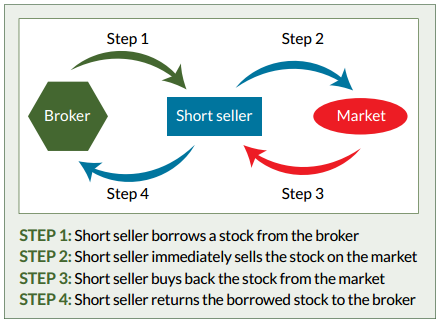
\includegraphics[height=0.36\textheight,keepaspectratio]{figures/slide38_img_flat.png}
\end{figure}
\end{frame}

% [src: 39]
\begin{frame}{Short Selling as a Bearish Signal}
My research shows that stocks with high \textbf{short interest ratio (SIR)} or \textbf{days-to-cover (DTC)} underperform significantly the next month.
\begin{description}
  \item[Short interest ratio] \# shares being shorted / total shares outstanding
  \item[Days-to-cover] \# shares being shorted / \# shares traded daily
\end{description}
\begin{columns}
\begin{column}{0.52\textwidth}
\begin{figure}
\centering
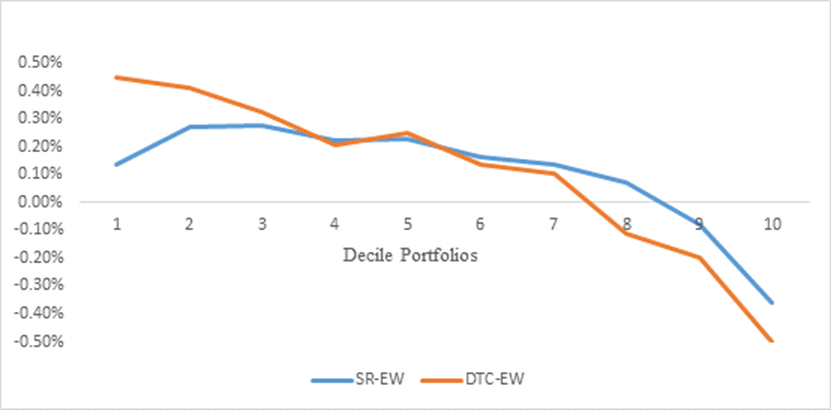
\includegraphics[height=0.44\textheight,keepaspectratio]{figures/slide39_img_flat.png}
\end{figure}
\end{column}
\begin{column}{0.44\textwidth}
\small
Source: Hong et al.\ (2016, Working Paper)
\vspace{0.4em}

WSJ coverage: \href{https://www.wsj.com/articles/beware-betting-against-short-sellers-1429290967}{``Beware Betting Against Short Sellers''}
\end{column}
\end{columns}
\end{frame}

% ============ STOCK RETURNS AND INDEXES ============

% [src: 40]
% Formula image (slide40_img.png) replaced by native math — content fully inferable from the extract.
\begin{frame}{Calculating Stock Returns}
The holding-period return on a stock over one period, $R_t$, divides into \textbf{capital gains} and \textbf{dividends}:
\[
R_t \;=\; \underbrace{\frac{P_t - P_{t-1}}{P_{t-1}}}_{\text{capital gain}} \;+\; \underbrace{\frac{D_t}{P_{t-1}}}_{\text{dividend return}}
\qquad\text{where } R_t = \frac{D_t + P_t - P_{t-1}}{P_{t-1}}
\]
\begin{itemize}
  \item $P_t$ = stock price at time $t$; \quad $D_t$ = dividends paid over $t-1$ to $t$
  \item $(P_t - P_{t-1})/P_{t-1}$ = capital gain over $t-1$ to $t$; \quad $D_t/P_{t-1}$ = return from dividends over $t-1$ to $t$
  \item This is the \textbf{pre-tax} return. The after-tax return multiplies each component by $(1 - \text{tax rate})$ --- usually different for capital gains versus dividends
\end{itemize}
\end{frame}

% [src: 41]
% slide41_img.png is blank in the extraction (all-black image) — dropped.
% slide41_img1.png (worked solution) replaced by the native worked solution below.
\begin{frame}{Calculating Stock Returns: Example}
An investor buys 10 shares of stock at \$55.10 and sells one year later at \$56.30, after collecting a \$0.30 dividend per share.
\begin{enumerate}
  \item \textbf{Pre-tax holding period return:}
  \[
  \text{HPR} = \frac{56.30 - 55.10 + 0.30}{55.10} = \frac{1.50}{55.10} = 2.72\%
  \]
  \item \textbf{After-tax HPR} (dividends taxed at 28\%, capital gains at 20\%):
  \[
  \text{HPR}_{\text{after-tax}} = \frac{1.20 \times (1-0.20) + 0.30 \times (1-0.28)}{55.10} = \frac{0.96 + 0.216}{55.10} = \frac{1.176}{55.10} = 2.13\%
  \]
\end{enumerate}
\end{frame}

% [src: 42]
\section{Stock Market Indexes}

% [src: 43, 44]
% slide44_img.jpg / slide44_img1.jpg: photos with no caption in the source deck; content not
% identifiable from the extraction — kept in a side-by-side display as in the original.
\begin{frame}{Stock Market Indexes}
A stock market index is the composite value of a group of secondary market-traded stocks; indexes provide information on broad stock market movement.
\begin{center}
\begin{columns}
\begin{column}{0.48\textwidth}
\centering
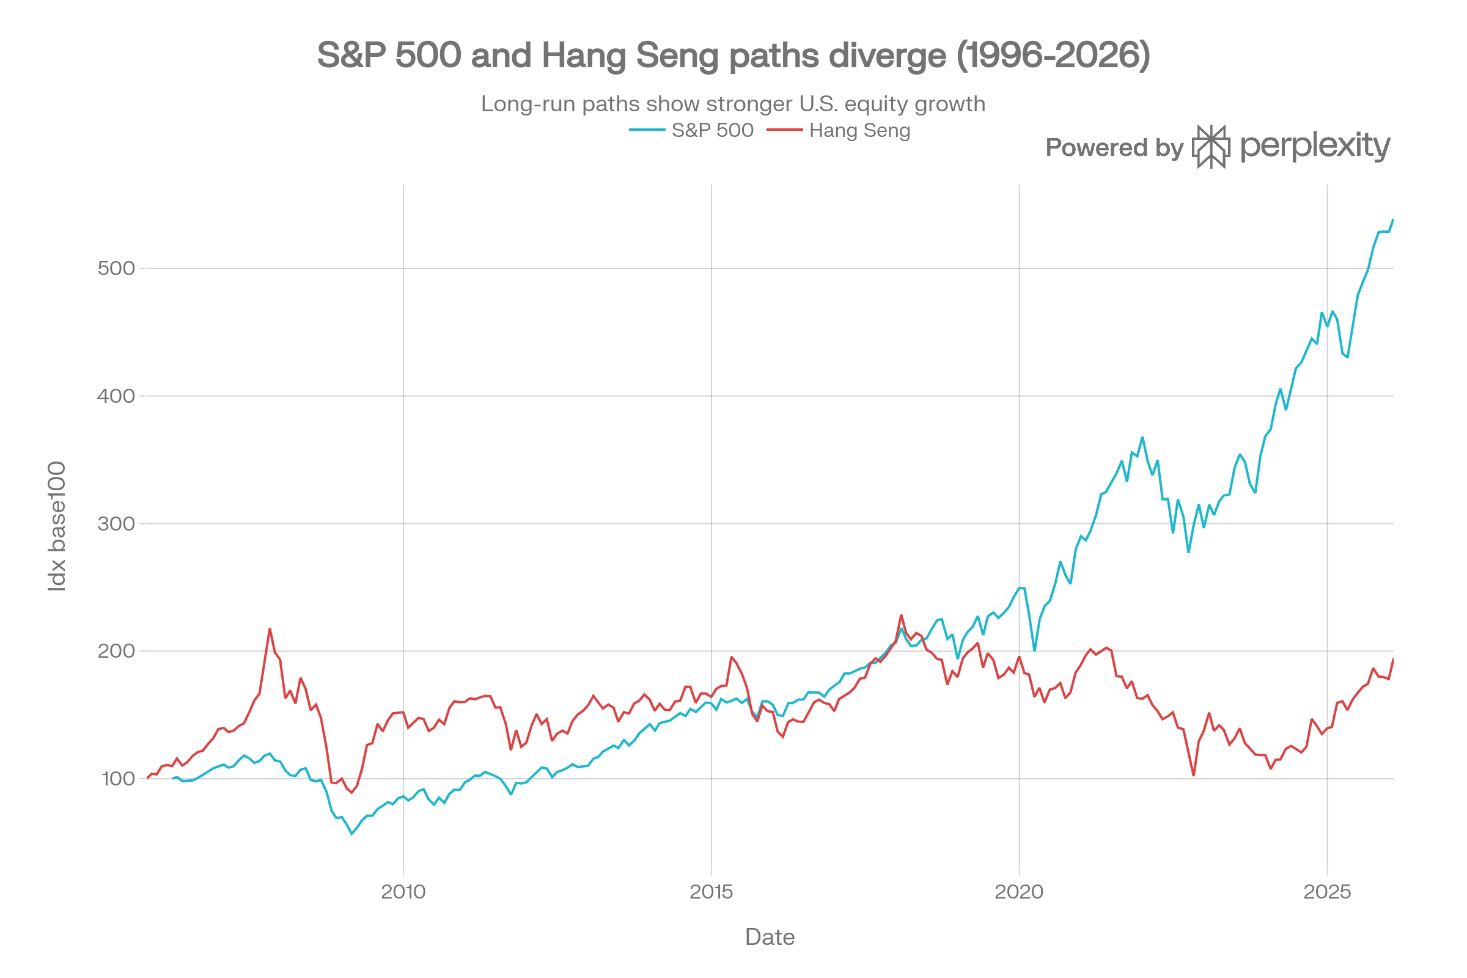
\includegraphics[height=0.32\textheight,keepaspectratio]{figures/slide43_img_flat.png}\\
{\scriptsize S\&P 500 vs.\ Hang Seng, indexed paths 1996--2026}
\end{column}
\begin{column}{0.48\textwidth}
\centering
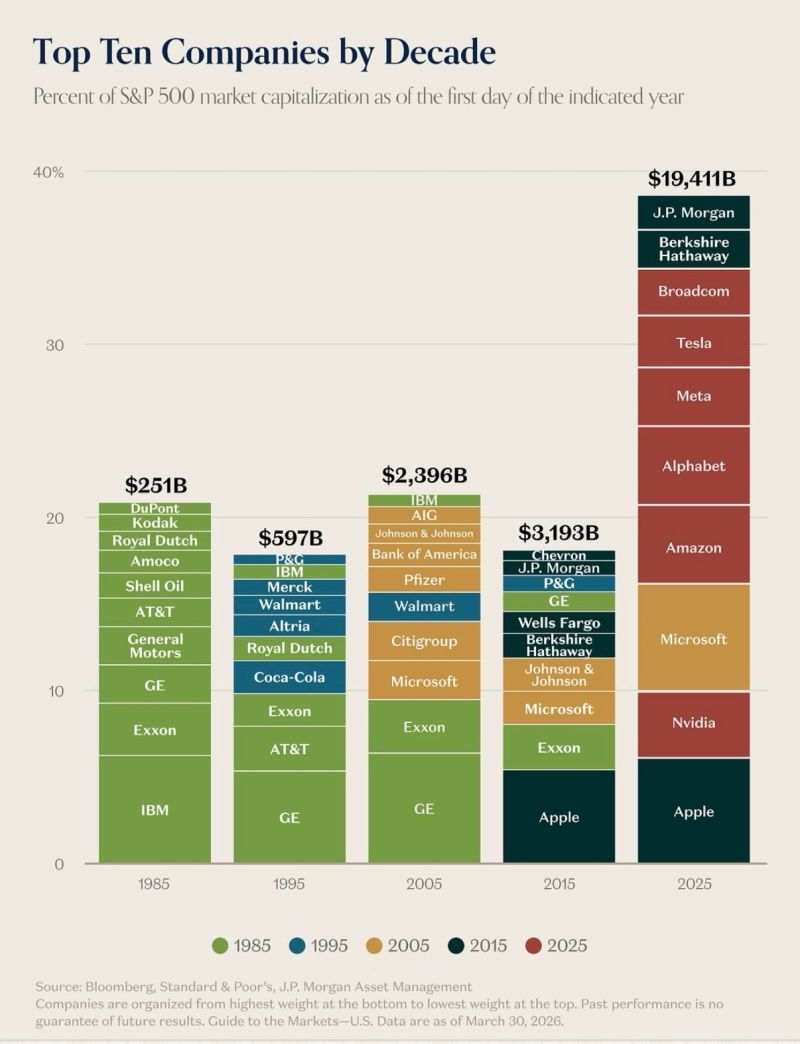
\includegraphics[height=0.32\textheight,keepaspectratio]{figures/slide44_img.jpg}\;
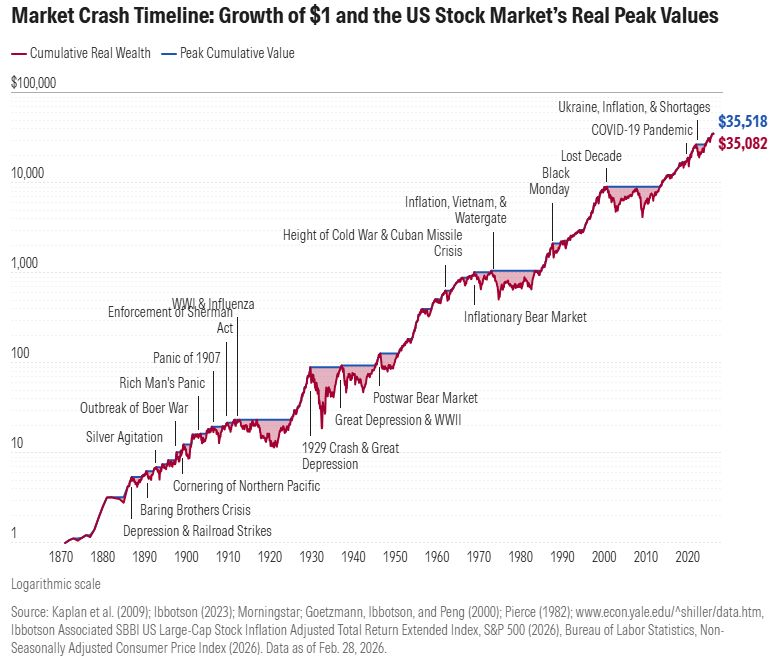
\includegraphics[height=0.32\textheight,keepaspectratio]{figures/slide44_img1.jpg}
\end{column}
\end{columns}
\end{center}
\end{frame}

% [src: 45]
\begin{frame}{Major Stock Market Indexes in the US}
\begin{description}
  \item[Dow Jones Industrial Average (DJIA)] One of the oldest, most well-known, and most frequently used indexes; 30 large blue-chip corporations. \textbf{Price-weighted}: each stock is weighted by its price per share --- the index is an average of the share prices of all companies
  \item[S\&P 500 Index (SPX)] A broad-based index of 500 firms representative of the US economy. \textbf{Market-cap weighted}: each stock is weighted by its total market capitalization (share price $\times$ number of shares outstanding)
\end{description}
\vspace{0.4em}
\textbf{Question:} what is the key difference between a price-weighted and a market-cap weighted index?
\end{frame}

% [src: 46]
\begin{frame}{Price-Weighted vs.\ Market-Cap Weighted Index: Example}
The market has three stocks, A, B, and C:
\begin{table}
\centering
\small
\begin{tabular}{lrrrrrr}
\toprule
 & \textbf{Initial price} & \textbf{Final price} & \textbf{Return} & \textbf{\# shares} & \textbf{Initial mkt cap} & \textbf{Final mkt cap} \\
\midrule
Stock A & \$30 & \$36 & 20\% & 700 & \$21,000 & \$25,200 \\
Stock B & \$100 & \$80 & $-$20\% & 100 & \$10,000 & \$8,000 \\
Stock C & \$70 & \$77 & 10\% & 200 & \$14,000 & \$15,400 \\
Total & \$200 & \$193 & & & \$45,000 & \$48,600 \\
\bottomrule
\end{tabular}
\end{table}
\begin{itemize}
  \item \textbf{Price-weighted}: initial index $= 200/3 = 66.7$; final index $= 193/3 = 64.3$; index return $= -3.5\%$
  \item \textbf{Market-cap weighted}: initial index $= 45{,}000/3 = 15{,}000$; final $= 48{,}600/3 = 16{,}200$; index return $= 8\%$
  \item \textbf{Question:} why do the two index returns differ?
\end{itemize}
\note{Price-weighted index = average prices of the individual stocks in the index; market-cap weighted index = average market capitalization of the individual stocks in the index.}
\end{frame}

% [src: 47]
\begin{frame}{Evolution of Sector Distribution in the Dow Jones}
\begin{table}
\centering
\scriptsize
\setlength{\tabcolsep}{4pt}
\begin{tabular}{lcccccccc}
\toprule
\textbf{Year} & \textbf{Info Tech} & \textbf{Fin.} & \textbf{Health} & \textbf{Cons.\ Disc.} & \textbf{Cons.\ Staples} & \textbf{Industrials} & \textbf{Energy/Mat.} & \textbf{Comm./Other} \\
\midrule
1928 & 0 & 1--2 & 0--1 & 3--5 & 4--6 & 15--18 & 6--8 & 1--2 \\
1950 & 0--1 & 2--3 & 1--2 & 4--6 & 5--7 & 12--15 & 5--7 & 2--3 \\
1980 & 1--2 (IBM) & 3--4 & 2--3 & 5--7 & 6--8 & 10--12 & 4--6 & 2--3 \\
2000 & 4--5 & 3--4 & 3--4 & 6--8 & 5--6 & 6--8 & 3--4 & 2--3 \\
2010 & 5--6 & 4--5 & 4 & 6--7 & 4--5 & 6--7 & 2--3 & 2 \\
2020 & 5 & 5--6 & 5 & 4--5 & 3--4 & 5--6 & 2--3 & 2--3 \\
Sept 2026 & 6 & 5 & 4 & 4 & 3 & 4 & 2 & 2 \\
\bottomrule
\end{tabular}
\end{table}
\note{Sept 2026 row counts (current GICS): IT 6 (AAPL, MSFT, IBM, CSCO, CRM, NVDA); Financials 5 (JPM, GS, V, AXP, TRV); Health Care 4 (UNH, JNJ, AMGN, MRK); Cons.\ Disc.\ 4 (AMZN, HD, MCD, NKE); Cons.\ Staples 3 (WMT, KO, PG); Industrials 4 (HON, BA, CAT, MMM); Energy/Materials 2 (CVX; SHW); Comm.\ Services 2 (DIS, GOOGL --- Alphabet replaced Verizon effective June 29, 2026, S\&P DJI). Sums to 30.}
\end{frame}

% [src: 48]
\begin{frame}{30 Stocks in the Dow Jones Industrial Average (Sept 2026)}
\begin{table}
\centering
\scriptsize
\setlength{\tabcolsep}{3pt}
\renewcommand{\arraystretch}{0.92}
\begin{tabular}{@{}lp{2.8cm}p{2.9cm}@{\hspace{0.5cm}}lp{2.8cm}p{2.9cm}@{}}
\toprule
\textbf{Ticker} & \textbf{Company} & \textbf{Industry} & \textbf{Ticker} & \textbf{Company} & \textbf{Industry} \\
\midrule
AAPL & Apple Inc. & Information technology & JNJ & Johnson \& Johnson & Pharmaceutical \\
AMGN & Amgen Inc. & Biopharmaceutical & JPM & JPMorgan Chase \& Co. & Financial services \\
AMZN & Amazon.com, Inc. & Retailing & KO & The Coca-Cola Company & Drink industry \\
AXP & American Express Co. & Financial services & MCD & McDonald's Corp. & Food industry \\
BA & The Boeing Company & Aerospace and defense & MMM & 3M Company & Conglomerate \\
CAT & Caterpillar Inc. & Construction equip. & MRK & Merck \& Co., Inc. & Pharmaceutical \\
CRM & Salesforce, Inc. & Information technology & MSFT & Microsoft Corporation & Information technology \\
CSCO & Cisco Systems, Inc. & Information technology & NKE & Nike, Inc. & Clothing industry \\
CVX & Chevron Corporation & Petroleum industry & NVDA & NVIDIA Corporation & Information technology \\
DIS & The Walt Disney Co. & Broadcasting, ent. & PG & Procter \& Gamble Co. & Fast-moving consumer goods \\
GOOGL & Alphabet Inc. & Interactive media \& services & SHW & Sherwin-Williams Co. & Specialty chemicals \\
GS & Goldman Sachs Group & Financial services & TRV & Travelers Companies & Insurance \\
HD & The Home Depot, Inc. & Home improvement retail & UNH & UnitedHealth Group & Managed health care \\
HON & Honeywell Intl.\ Inc. & Conglomerate & V & Visa Inc. & Financial services \\
IBM & Intl.\ Business Machines & Information technology & WMT & Walmart Inc. & Retailing \\
\bottomrule
\end{tabular}
\end{table}
\note{Roster as of Sept 2026 (S\&P DJI). Alphabet (GOOGL) replaced Verizon (VZ) effective June 29, 2026. Earlier confirmed changes: Nvidia and Sherwin-Williams joined November 8, 2024 (replacing Intel and Dow Inc.); Amazon joined February 26, 2024 (replacing Walgreens). Amgen has been a member since August 2020.}
\end{frame}

% [src: 49]
\begin{frame}{Issues with the S\&P 500 Index}
Growing dominance of the \textbf{Magnificent 7} stocks --- Apple, Microsoft, Amazon, Nvidia, Alphabet/Google, Meta, and Tesla --- in the S\&P 500 index.
\begin{figure}
\centering

\includegraphics[height=0.62\textheight,keepaspectratio]{figures/slide49_img_flat.png}
\end{figure}
\note{If you're invested in broad S\&P 500 index funds (like SPY), you're already exposed to this concentration --- rewarding in bull markets but it amplifies volatility. Some investors are shifting toward equal-weight S\&P 500 strategies to reduce reliance on the top names. As of September 2026, the Magnificent 7 (Apple, Microsoft, Nvidia, Alphabet, Amazon, Meta, Tesla) continue to account for a disproportionate share of S\&P 500 market cap.}
\end{frame}

% [src: 50]
\begin{frame}{Other Major Stock Market Indexes}
\begin{columns}
\begin{column}{0.48\textwidth}
\textbf{US indexes}
\begin{itemize}
  \item \textbf{NASDAQ Composite (COMP)}: market-cap weighted index of all stocks traded on the Nasdaq stock exchange
  \item \textbf{Russell 3000}: market-cap weighted index of the 3,000 largest US-traded stocks --- about 97\% of all US-incorporated equity securities
\end{itemize}
\end{column}
\begin{column}{0.48\textwidth}
\textbf{Major indexes outside the US}
\begin{itemize}
  \item UK: FTSE 100
  \item Singapore: Straits Times Index (STI)
  \item Japan: Nikkei 225
  \item China: Shanghai Composite (SHCOMP)
  \item Hong Kong: Hang Seng Index (HSI)
\end{itemize}
\end{column}
\end{columns}
\end{frame}

% [src: 51]
\begin{frame}{Global Equity Market Cap}
\begin{figure}
\centering

\includegraphics[height=0.72\textheight,keepaspectratio]{figures/slide51_img_flat.png}
\end{figure}
\end{frame}

% [src: 52]
% slide52_img.emf (native chart) converted to PNG (slide52_img.png) via GDI+ — keep both files.
\begin{frame}{Is the Stock Market a Leading Economic Indicator?}
\begin{itemize}
  \item An increase (decrease) in stock market indexes today potentially signals the market's expectation of higher (lower) corporate dividends and profits and, in turn, higher (lower) economic growth
  \item One of the leading economic indicators used by the Fed
\end{itemize}
\begin{figure}
\centering

\includegraphics[height=0.56\textheight,keepaspectratio]{figures/slide52_img_flat.png}
\end{figure}
\end{frame}

% [src: 53]
% TODO: recreate chart — the source deck has a NATIVE CHART (no figure extracted); Shiller CAPE
% ratio chart from Robert Shiller's website needs to be recreated or screenshotted.
\begin{frame}{Is the US Stock Market in a Bubble Now?}
\begin{center}
\small Source: Robert Shiller's website
\end{center}
\note{Only 2 periods in history have we seen a higher P/E ratio than today's P/E: 1929 and 2000. The stock market crashed subsequently in both.}
\end{frame}

% ============ REGULATION ============

% [src: 54]
\section{Regulation of the Stock Market}

% [src: 55]
\begin{frame}{US Stock Market Regulations}
\begin{description}
  \item[SEC --- Securities and Exchange Commission] The primary regulator of US stock markets. Promotes full disclosure of information on securities and fair treatment of investors; enforces the Securities Act of 1933 and the Securities Exchange Act of 1934; prosecutes illegal insider trading
  \item[FINRA --- Financial Industry Regulatory Authority] The regulator for all US securities firms: oversees brokers and dealers, examines securities firms and promulgates rules, enforces federal securities laws, and conducts dispute arbitration
\end{description}
\end{frame}

% [src: 56, 57]
\begin{frame}{The SFC in Hong Kong}
The \textbf{Securities and Futures Commission (SFC)} is an independent statutory body set up in 1989 to regulate Hong Kong's securities and futures markets. Its investigative, remedial, and disciplinary powers derive from the \textbf{Securities and Futures Ordinance (SFO)} and subsidiary legislation. Operationally independent of the Government of the HKSAR; funded mainly by transaction levies and licensing fees.
\vspace{0.3em}
\begin{itemize}
  \item \textbf{Protecting investors}: safeguard the investing public through fair treatment, transparency, and adequate disclosure
  \item \textbf{Maintaining fair, orderly, and efficient markets}
  \item \textbf{Licensing and supervision of intermediaries}
  \item \textbf{Enforcement and discipline}: investigate suspected breaches of securities laws
  \item \textbf{Promoting market development and education}: encourage the orderly growth and international competitiveness of HK's financial markets; investor education via resources, alerts, and campaigns
  \item \textbf{Regulation of products and activities}: authorize and oversee collective investment schemes (e.g., mutual funds, unit trusts)
\end{itemize}
\end{frame}

% [src: 58, 59]
\begin{frame}{Key Takeaways}
\begin{description}
  \item[Stocks] Ownership (common stock) with voting rights \& residual claim; preferred stock has fixed dividends \& priority but usually no vote
  \item[Primary market] Firms raise capital via investment banks (firm commitment vs.\ best efforts). IPO anomalies: significant underpricing (high first-day returns) followed by long-run underperformance (3--5 years); reasons include winner's curse, bank conflicts, market timing
  \item[Secondary market] NYSE: auction market with designated market makers; NASDAQ: dealer market with multiple market makers. Market orders = immediate execution; limit orders = price control. Short selling bets on price decline via borrowed shares; high short interest predicts negative returns
  \item[Returns and indexes] Total return = capital gains + dividends. Price-weighted (DJIA): higher-priced stocks have more influence; market-cap weighted (S\&P 500): larger companies have more influence. Indexes are leading economic indicators
  \item[Regulation] SEC (US) / SFC (HK): ensure full disclosure, fair trading, and prosecute insider trading
\end{description}
\end{frame}

\end{document}
